\documentclass[preview]{standalone}

\usepackage{amsmath}
\usepackage{amssymb}
\usepackage{stellar}
\usepackage{definitions}
\usepackage{tikz}

\usetikzlibrary{automata,arrows}

\begin{document}

\id{linearalgebra-exercises-batch-11}
\genpage

\section{Exercises}

\begin{snippetexercise}{linear-algebra-batch-11-ex-1}{}
    \todo
\end{snippetexercise}

\begin{snippetsolution}{linear-algebra-batch-11-ex-1-sol}{}
    \todo
\end{snippetsolution}

\begin{snippetexercise}{linear-algebra-batch-11-ex-2}{}
    \todo
\end{snippetexercise}

\begin{snippetsolution}{linear-algebra-batch-11-ex-2-sol}{}
    \todo
\end{snippetsolution}

\begin{snippetexercise}{linear-algebra-batch-11-ex-3}{}
    \todo
\end{snippetexercise}

\begin{snippetsolution}{linear-algebra-batch-11-ex-3-sol}{}
    \todo
\end{snippetsolution}

\begin{snippetexercise}{linear-algebra-batch-11-ex-4}{}
    \todo
\end{snippetexercise}

\begin{snippetsolution}{linear-algebra-batch-11-ex-4-sol}{}
    \todo
\end{snippetsolution}

\begin{snippetexercise}{linear-algebra-batch-11-ex-5}{}
    \todo
\end{snippetexercise}

\begin{snippetsolution}{linear-algebra-batch-11-ex-5-sol}{}
    \todo
\end{snippetsolution}

\begin{snippetexercise}{linear-algebra-batch-11-ex-6}{}
    \todo
\end{snippetexercise}

\begin{snippetsolution}{linear-algebra-batch-11-ex-6-sol}{}
    \todo
\end{snippetsolution}

\begin{snippetexercise}{linear-algebra-batch-11-ex-7}{}
    \todo
\end{snippetexercise}

\begin{snippetsolution}{linear-algebra-batch-11-ex-7-sol}{}
    \todo
\end{snippetsolution}

\begin{snippetexercise}{linear-algebra-batch-11-ex-8}{}
    \todo
\end{snippetexercise}

\begin{snippetsolution}{linear-algebra-batch-11-ex-8-sol}{}
    \todo
\end{snippetsolution}

\begin{snippetexercise}{linear-algebra-batch-11-ex-9}{}
    \todo
\end{snippetexercise}

\begin{snippetsolution}{linear-algebra-batch-11-ex-9-sol}{}
    \todo
\end{snippetsolution}

\begin{snippetexercise}{linear-algebra-batch-11-ex-10}{}
    \todo
\end{snippetexercise}

\begin{snippetsolution}{linear-algebra-batch-11-ex-10-sol}{}
    \todo
\end{snippetsolution}

\begin{snippetexercise}{linear-algebra-batch-11-ex-11}{}
    \todo
\end{snippetexercise}

\begin{snippetsolution}{linear-algebra-batch-11-ex-11-sol}{}
    \todo
\end{snippetsolution}

\begin{snippetexercise}{linear-algebra-batch-11-ex-12}{}
    \todo
\end{snippetexercise}

\begin{snippetsolution}{linear-algebra-batch-11-ex-12-sol}{}
    \todo
\end{snippetsolution}

\begin{snippetexercise}{linear-algebra-batch-11-ex-13}{}
    \todo
\end{snippetexercise}

\begin{snippetsolution}{linear-algebra-batch-11-ex-13-sol}{}
    \todo
\end{snippetsolution}

\begin{snippetexercise}{linear-algebra-batch-11-ex-14}{}
    A particle \(P\) can be found, at every discrete time \(t\geq 0\), in a state \(A\)
    or \(B\). The probability of \(P\) switching state are given in the following diagram:
    \begin{center}
        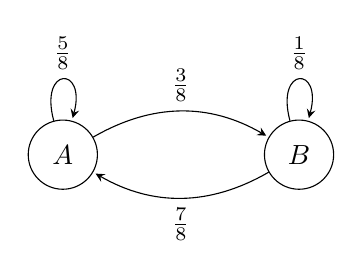
\begin{tikzpicture}[->,>=stealth,shorten >=1pt,auto,node distance=3cm]
        % nodi
        \node[state] (A)                    {$A$};
        \node[state] (B) [right of=A]      {$B$};
        % archi
        \path
            (A) edge[loop above]   node{$\tfrac{5}{8}$} (A)
                edge[bend left]    node{$\tfrac{3}{8}$} (B)
            (B) edge[loop above]   node{$\tfrac{1}{8}$} (B)
                edge[bend left]    node{$\tfrac{7}{8}$} (A);
        \end{tikzpicture}
    \end{center}
    For \(t=0\), the particle is equally likely to be in state \(A\) or \(B\). Find
    the probabilities of each state for \(t=1\) and for \(t = n\) when \(n\to\infty\).
\end{snippetexercise}

\begin{snippetsolution}{linear-algebra-batch-11-ex-14-sol}{}
    \todo
\end{snippetsolution}

\begin{snippetexercise}{linear-algebra-batch-11-ex-15}{}
    \todo
\end{snippetexercise}

\begin{snippetsolution}{linear-algebra-batch-11-ex-15-sol}{}
    \todo
\end{snippetsolution}

\begin{snippetexercise}{linear-algebra-batch-11-ex-16}{}
    \todo
\end{snippetexercise}

\begin{snippetsolution}{linear-algebra-batch-11-ex-16-sol}{}
    \todo
\end{snippetsolution}

\begin{snippetexercise}{linear-algebra-batch-11-ex-17}{}
    \todo
\end{snippetexercise}

\begin{snippetsolution}{linear-algebra-batch-11-ex-17-sol}{}
    \todo
\end{snippetsolution}

\end{document}